% !TEX root = thesis.tex
\documentclass[11pt, % MIT requirements, at least 11 pt
            %    draft,
            %    draftversion, % prints draft on front page
               twoside,
               letterpaper,openright]{uwthesis}

\hypersetup{
  pdfinfo={
    Title={Some long title about some interesting subject},
    Author={John Doe},
    Subject={PhD Thesis},
    Keywords={MIT, some interesting subject}
  }
}

\author{John Doe}

\include{preamble}

\addbibresource{bibliography.bib}

\begin{document}
  \chapterstyle{uw}
  \pagestyle{uw}
  \maxsecnumdepth{subsection}

    \mainmatter

      \begin{whole}
        \maketitle
      \end{whole}

      {\pagestyle{plain}%
      \printabstract{chapters/0_abstract}%
      }
      \cleardoublepage

      \include{dedication}

      \cleardoublepage
      \pdfbookmark[chapter]{Acknowledgements}{acknowledgements}%

\chapter*{Acknowledgements}


\lipsum[1]
Thank you! \\

\vspace{1em}
\mbox{} \hfill \textit{Author}\\
\mbox{} \hfill Seattle, Washington\vspace{-0.35pc}\\
\mbox{} \hfill June 2025


      \cleardoublepage%
      \pdfbookmark{\contentsname}{toc}%
      {\SingleSpacing\tableofcontents*}

      \cleardoublepage

      {\phantomsection%
      \SingleSpacing%
      \input{nomenclature.tex}%
      \addcontentsline{toc}{chapter}{Nomenclature}%
      \printnomenclature[0.8in]%
      }%

      \cleardoublepage

      {\phantomsection%
      \SingleSpacing%
      \printglossary[title=Acronyms,type=\acronymtype]}

      \cleardoublepage

      {\RaggedRight\SingleSpacing\listoffigures\cleardoublepage
      \listoftables}

      \include{chapters/1_intro}

      \include{chapters/2_methods}

      % !TEX root = ../thesis.tex
\chapter{Results}\label{chap:results}

\lipsum

\begin{items}
\item Item 1
\item Item 2
\item Item 3
\end{items}

\lipsum

\begin{enum}
\item Enum 1
\item Enum 2
\item Enum 3
\end{enum}

\lipsum[1-8]


      % !TEX root = ../thesis.tex
\chapter{Conclusions and Outlook}\label{chap:conclusion}

This thesis presented some stuff.
\lipsum[2-3]

\begin{figure}[ht]
    \begin{fullwidthfig}
      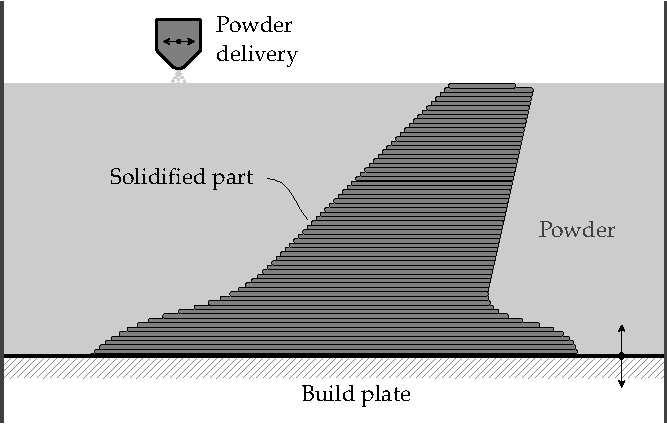
\includegraphics[width=\fullwidth]{figures/example/powder_based}
    \end{fullwidthfig}
    \captionb[Shorter caption for in the LOF.]{This is some exciting figure, generated in Tikz. Note how the caption is below the figure.}{fig:tikz}
 \end{figure}

\lipsum[2-3]


      {\SingleSpacing\printbibliography}

      \addcontentsline{toc}{part}{\appendixtocname}
      \appendixpage*

      \def\chaptername{Appendix}

      \bookmarksetup{startatroot}
      \appendix
      \include{appendices/app}

      {\SingleSpacing\small\printindex}

      \newpage  \clearpage \mbox{}
      {%
\thispagestyle{empty}%
\SingleSpacing%
\small%
\vfill%
\pdfbookmark[chapter]{Colophon}{colophon}%
\section*{Colophon}
% \noindent This thesis has been typeset using \LaTeX{} in the Palatino font.
\noindent This thesis has been typeset using \LaTeX{}, and compiled using \texttt{pdflatex}, based on the template by Max Opgenoord (\href{https://github.com/mopg/uw-phd-thesis}{github.com/mopg/uw-phd-thesis}).
% Minion Pro is used as both the text and display typeface. The sans-serif text uses the \textsf{Myriad Pro} typeface,
Palatino is used as the text typeface, % comment this line if you end up using Minion Pro
whereas monospaced text is typeset in \texttt{Bitstream Vera Mono}.
\mbox{}\vspace{0.5pc}\\
\noindent Several books have influenced the style, typography, and graphic design of this thesis, in particular:
\begin{itemize}
  \item[] Edward Tufte's \textit{Beautiful Evidence} (2006)
  \item[] Jean-Luc Doumont's \textit{Trees, Maps, and Theorems} (2009)
  \item[] Robert Bringhurst's \textit{Elements of Typography} (1992)
\end{itemize}
\vspace{0.75pc}% \mbox{}\\

{\SingleSpacing\noindent\textit{Very Long }\\
\textit{thesis title}\vspace{0.25pc}\\}
Author, June 2025 \vspace{1.25pc}\\
\noindent \textcopyright\ John Doe 2025. All rights reserved.\vspace{1pc} \\
}


      \newpage  \clearpage \mbox{} \thispagestyle{empty}
      \newpage  \clearpage \mbox{} \thispagestyle{empty}%
      {%
        \begin{tikzpicture}[remember picture,overlay]
        \node[at=(current page.south),gray,anchor=south,yshift=1in,text width=0.5\paperwidth,align=center]{
            \footnotesize%
            \SingleSpacing%
            \begin{minipage}{\linewidth}
                  \centering
                  Ph.D. Dissertation\\
                  John Doe\vskip0.5em
                  \textit{Some very long title}\\
                  \textit{about some interesting topic}\vskip0.5em
                  -- \textsc{mmxxv} --
            \end{minipage}};
        \end{tikzpicture}
      }

\end{document}
